\subsubsection{SymTime and the \texorpdfstring{S$^2$}{S2}Generator
series--symbol prior}

\paragraph{Purpose and position in this review.}
\citet{wang2025symtime} introduce S$^2$Generator to produce paired symbolic
expressions and multivariate time series at the scale required to pretrain
SymTime. The paper belongs in this subsection because its learned output is a
general-purpose time-series representation for downstream analysis. The
symbolic expression acts as a second, semantically aligned view during
pretraining. This differs from the symbolic-regression methods in
Section~1.2, whose learned output is the equation itself.

\paragraph{The complete generated object.}
S$^2$Generator first samples a vector-valued algebraic map
$\mathbf f_{\mathrm{S^2}}:\mathbb R^{M_{\mathrm{S^2}}}\rightarrow
\mathbb R^{N_{\mathrm{S^2}}}$ and then samples the input trajectories to which
that map is applied. In the common notation of Table~\ref{tab:notation}, one
example is

\begin{equation}
\begin{aligned}
x_{j,1:T_{\mathrm{S^2}}}
  &=G_{X,j}(\boldsymbol\eta_j;\boldsymbol\theta_j),
  &&j=1,\ldots,M_{\mathrm{S^2}},\\
y_{i,t}
  &=f_i(x_{1,t},\ldots,x_{M_{\mathrm{S^2}},t}),
  &&i=1,\ldots,N_{\mathrm{S^2}},\quad
    t=1,\ldots,T_{\mathrm{S^2}}.
\end{aligned}
\label{eq:s2-complete-generator}
\end{equation}

Here $G_{X,j}$ denotes the sampled stochastic process for input channel $j$,
$\boldsymbol\theta_j$ its parameters, and $\boldsymbol\eta_j$ its realized
random innovations. The full series generator is consequently the composition
$\mathbf g_{\mathrm{S^2}}=\mathbf f_{\mathrm{S^2}}\circ\mathbf G_X$.
This separation is essential: $\mathbf f_{\mathrm{S^2}}$ describes which
current input variables are algebraically transformed into each current
output, whereas $\mathbf G_X$ supplies the temporal behavior of those inputs.

\paragraph{How the expression trees are sampled.}
The generator exhaustively traverses
$M_{\mathrm{S^2}}\in\{1,\ldots,6\}$ and
$N_{\mathrm{S^2}}\in\{1,\ldots,12\}$ rather than randomly favoring some
input--output dimensions. It samples one separate tree $f_i$ for every output
channel and applies the following construction \citep{wang2025symtime}:

\begin{enumerate}
    \item draw the number of binary nodes
    $b\sim\mathcal U\{b_{\min},\ldots,b_{\max}\}$ and label them uniformly
    from $\{+,-,\times\}$;

    \item combine those nodes into a full binary-tree skeleton. The released
    implementation uses the same open-slot/completion-count sampler found in
    the Transformer symbolic-regression generator family: a binary node
    consumes one open position and creates two, and the next insertion
    position is sampled from the number of valid completions;

    \item choose $m\sim\mathcal U\{1,\ldots,M_{\mathrm{S^2}}\}$ input
    variables for leaves and add random constants to the remaining leaf
    positions needed to complete the tree;

    \item draw $u\sim\mathcal U\{u_{\min},\ldots,u_{\max}\}$ and insert unary
    nodes at random valid positions. The library is
    $\{\operatorname{inv},|\cdot|,(\cdot)^2,(\cdot)^3,\sqrt{\cdot},
    \sin,\cos,\tan,\arctan,\log,\exp\}$;

    \item apply random affine transformations $z\mapsto az+b$ to selected
    variable leaves and unary outputs, increasing coefficient and offset
    diversity without changing the sampled topology.
\end{enumerate}

For example, the tree in Figure~\ref{fig:s2-tree-and-series} represents
$f_i(\mathbf x)=\sin(x_1)+x_2x_3$. Its binary skeleton has a sum at the root
and a product in the right branch; the sine is inserted afterward as a unary
node. The actual generator may wrap these nodes in the sampled affine
transformations.

\begin{figure}[H]
\centering
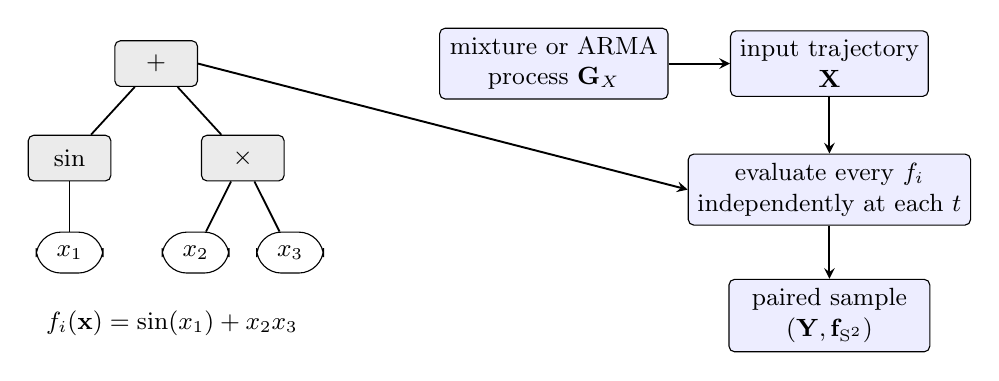
\begin{tikzpicture}[
    operator/.style={draw,rounded corners=2pt,fill=black!8,
        minimum width=1.05cm,minimum height=0.58cm,align=center,font=\small},
    leaf/.style={draw,rounded corners=9pt,fill=white,
        minimum width=0.85cm,minimum height=0.52cm,align=center,font=\small},
    block/.style={draw,rounded corners=2pt,fill=blue!7,
        minimum width=2.55cm,minimum height=0.72cm,align=center,font=\small},
    flow/.style={->,>=stealth,draw,line width=0.7pt},
    branch/.style={draw,line width=0.65pt}
]
    \node[operator] (add) at (-5.4,2.35) {$+$};
    \node[operator] (sin) at (-6.5,1.15) {$\sin$};
    \node[operator] (mul) at (-4.3,1.15) {$\times$};
    \node[leaf] (x1) at (-6.5,-0.05) {$x_1$};
    \node[leaf] (x2) at (-4.9,-0.05) {$x_2$};
    \node[leaf] (x3) at (-3.7,-0.05) {$x_3$};
    \draw[branch] (add)--(sin); \draw[branch] (add)--(mul);
    \draw[branch] (sin)--(x1);
    \draw[branch] (mul)--(x2); \draw[branch] (mul)--(x3);
    \node[font=\small,align=center] at (-5.2,-0.95)
        {$f_i(\mathbf x)=\sin(x_1)+x_2x_3$};

    \node[block,minimum width=2.9cm] (input) at (-0.35,2.35)
        {mixture or ARMA\\process $\mathbf G_X$};
    \node[block,minimum width=2.35cm] (X) at (3.15,2.35)
        {input trajectory\\$\mathbf X$};
    \node[block,minimum width=3.2cm] (f) at (3.15,0.75)
        {evaluate every $f_i$\\independently at each $t$};
    \node[block] (pair) at (3.15,-0.85)
        {paired sample\\$(\mathbf Y,\mathbf f_{\mathrm{S^2}})$};
    \draw[flow] (input)--(X);
    \draw[flow] (X)--(f);
    \draw[flow] (add.east) -- (f.west);
    \draw[flow] (f)--(pair);
\end{tikzpicture}
\caption{S$^2$Generator separates the sampled symbolic transformation from
the process that supplies its temporal inputs. The displayed tree acts on one
aligned input vector $\mathbf x_t$ at a time; mixture or ARMA sampling creates
the trajectory across $t$.}
\label{fig:s2-tree-and-series}
\end{figure}

\paragraph{How temporal inputs and outputs are produced.}
Every input channel is drawn either from a random finite mixture of Gaussian
or uniform distributions, or from a random-parameter ARMA$(p,q)$ process. In
the latter branch, the common notation gives

\begin{equation}
x_{j,t}=\sum_{r=1}^{p}a_{j,r}x_{j,t-r}
          +\eta_{j,t}
          -\sum_{s=1}^{q}\vartheta_{j,s}\eta_{j,t-s}.
\label{eq:s2-arma-input}
\end{equation}

The orders and coefficients are sampled within the bounds reported by the
paper, with constraints intended to favor stationary AR dynamics. Mixture
inputs provide varied marginal distributions; ARMA inputs additionally carry
serial dependence. Each channel of $\mathbf X$ is standardized, all trees are
evaluated pointwise according to Equation~\eqref{eq:s2-complete-generator},
and samples outside an operator's valid domain or with
$|y_{i,t}|>10^4$ are rejected. The released corpus contains 40 million
series--symbol pairs with a cumulative sequence length of 50 billion. For
fixed tree size, channel counts, mixture size, and ARMA orders, the authors'
analysis and timing experiment show generation cost approximately linear in
$T_{\mathrm{S^2}}$. Oversized random trees narrow valid domains and lower the
acceptance rate, which motivates the paper's bounded operator library.

\paragraph{How SymTime uses the pair.}
The time-series branch is a six-layer Transformer trained to reconstruct
masked non-overlapping patches. The symbolic branch is a six-layer DistilBERT
trained with masked-language modeling. Bidirectional series--symbol contrastive
loss aligns the two \texttt{[CLS]} representations, while momentum encoders
provide soft distillation targets. The total objective combines masked time
modeling, masked language modeling, contrastive alignment, and momentum
distillation. Fine-tuning uses the temporal encoder for long- and short-term
forecasting, classification, imputation, and anomaly detection. Thus, the
paired equation teaches a semantic representation; SymTime's decoder target
in downstream forecasting remains a future series rather than a recovered
prefix expression.

\paragraph{What is reused and what is new.}
Table~\ref{tab:s2-vs-symbolic-regression} shows that the tree data structure
and its random construction follow the established symbolic-regression
family. S$^2$Generator's contribution is the large-scale pairing of a sampled
algebraic map with a temporally structured multivariate stimulus, exhaustive
input/output dimensional coverage, and cross-modal pretraining on the
resulting series--symbol pairs.

\begin{table}[H]
\centering
\footnotesize
\renewcommand{\arraystretch}{1.06}
\begin{tabular}{@{}p{0.17\textwidth}p{0.27\textwidth}p{0.25\textwidth}p{0.23\textwidth}@{}}
\toprule
Work & Meaning of the sampled tree & Source of temporal dependence & Learned output \tabularnewline
\midrule
D'Ascoli et al. & Recurrence $u_n=F_{\mathcal T}(n,u_{n-1},\ldots)$ & Lagged sequence values are leaves of the tree & Recovered recurrence \tabularnewline
Me\v{z}nar et al. & General algebraic expression represented in a learned latent tree space & Defined by the later application of the expression & Expression optimized in latent space \tabularnewline
Bendinelli et al. & Static map $y=e(\mathbf x)$ paired with numerical support and hypotheses & A time-series adaptation would encode lags as input features & Recovered expression constrained by hypotheses \tabularnewline
ODEFormer & Vector field $\dot{\mathbf x}=\mathbf f(\mathbf x)$ & Numerical integration of the sampled field & Recovered differential equation \tabularnewline
S$^2$Generator and SymTime & Pointwise multivariate map $\mathbf y_t=\mathbf f_{\mathrm{S^2}}(\mathbf x_t)$ & Mixture or ARMA process $\mathbf G_X$ generates the input trajectory & Time-series representation aligned with symbolic semantics \tabularnewline
\bottomrule
\end{tabular}
\caption{The same broad unary--binary tree machinery receives different
temporal semantics and supports different learning objectives.}
\label{tab:s2-vs-symbolic-regression}
\end{table}

\paragraph{Explanation ground truth available to this thesis.}
The retained expression directly defines a contemporaneous structural mask

\begin{equation}
M^{\mathrm{S^2}}_{i,j}
=\mathbb I[x_j\text{ occurs in }f_i]
\label{eq:s2-structural-mask}
\end{equation}

and, wherever the sampled expression is differentiable, an exact local signed
sensitivity

\begin{equation}
J^{\mathrm{S^2}}_{i,j,t}
=\left.
\frac{\partial f_i(\mathbf x)}{\partial x_j}
\right|_{\mathbf x=\mathbf x_t}.
\label{eq:s2-local-jacobian}
\end{equation}

These references explain how the aligned stimulus $\mathbf x_t$ produces
$\mathbf y_t$. A variable--lag forecasting reference additionally requires
the ARMA mechanism in $\mathbf G_X$ and propagation of its lagged dependence
through $\mathbf f_{\mathrm{S^2}}$. Retaining both halves of
Equation~\eqref{eq:s2-complete-generator} would therefore strengthen the
proposed benchmark: the expression tree records the nonlinear cross-variable
transformation, while the sampled input-process record supplies temporal
memory. Extending the tree leaves themselves with
$\operatorname{LAG}(j,\ell)$ or recursive feedback would make temporal
dependencies explicit in one canonical mechanism.

The paper evaluates synthetic-data coverage using stationarity,
forecastability, mean FFT power, permutation entropy, seasonality, and trend.
It evaluates SymTime through downstream predictive tasks and representation
ablations. Direct equation-recovery accuracy and agreement
between XAI maps and generator-derived explanations lie outside that reported
protocol. For this thesis, S$^2$Generator is therefore chiefly a scalable
generator architecture and paired-data precedent; Equations
\eqref{eq:s2-structural-mask}--\eqref{eq:s2-local-jacobian} show the additional
references that can be derived once all sampled mechanisms are retained.

The official implementations are available in the S$^2$Generator repository
(\url{https://github.com/wwhenxuan/S2Generator}) and the SymTime repository
(\url{https://github.com/wwhenxuan/SymTime}).

\begin{table}[H]
\centering
\footnotesize
\renewcommand{\arraystretch}{1.04}
\begin{tabular}{@{}p{0.17\textwidth}p{0.31\textwidth}p{0.43\textwidth}@{}}
\toprule
Method & Retained synthetic mechanism & Scaling strategy and use in this thesis \\
\midrule
KernelSynth & Composite GP kernel $\kappa_\star$ & CPU-parallel GP draws and Arrow/LZ4 storage; supplies a covariance mechanism and exact conditional-mean gradient. \\
Chronos-2 & Base generator plus contemporaneous or sequential multivariatization & Patching, time/group attention, and a direct quantile head; motivates multivariate, lead--lag, and covariate-informed tasks. \\
TempoPFN and Toto 2.0 & Generator identity, sampled parameters, regimes, and augmentation chain & Mixed CPU/GPU priors plus Toto's CPM, u-$\mu$P, and FSDP2; motivates difficulty by regime, change point, long memory, and noise. \\
TimePFN/LMC-Synth & Latent GP kernels and Dirichlet mixing matrix & CPU-parallel sampling and channel-mixing attention; supplies known cross-channel covariance and a dense Jacobian reference. \\
S$^2$Generator and SymTime & Pointwise expression trees plus mixture/ARMA input processes & Approximately linear cost in sequence length for fixed mechanism size and paired series--symbol pretraining; supplies contemporaneous structure and a local Jacobian, while the retained input process adds temporal ground truth. \\
\bottomrule
\end{tabular}
\caption{Relationship between the synthetic pretraining methods, their
high-throughput implementations, and the proposed explanation benchmark.}
\label{tab:foundation-synthetic-comparison}
\end{table}

